\documentclass[letterpaper]{article}

%% Language and font encodings
\usepackage[english]{babel}

%\usepackage[utf8]{inputenc}
\usepackage[T1]{fontenc}
%\usepackage{indentfirst}

%% Sets page size and margins
\usepackage[letterpaper,top=1in,bottom=1in,left=1in,right=1in,margin=1in]{geometry}

%% Useful packages
\usepackage{etoolbox}
\usepackage{setspace}
\usepackage{subcaption}
\usepackage{float}
\usepackage{amsmath}
\usepackage{svrsymbols}
\usepackage{titletoc}
\usepackage[titles]{tocloft}
\usepackage{tikz-feynman}
\tikzfeynmanset{compat=1.1.0}

%%Quote configuration%%
\AtBeginEnvironment{quote}{\singlespacing\small}

%%Formatting Contents%%
\usepackage{titlesec}
\titleformat{\section}[block]{\color{black}\Large\bfseries\filcenter}{}{1em}{}
\renewcommand{\cftsecfont}{\color{black}\normalfont}
\renewcommand{\cftsecpagefont}{\color{black}\normalfont}
\newcommand*{\BeginNoToc}{%
 \addtocontents{toc}{%
   \edef\protect\SavedTocDepth{\protect\the\protect\value{tocdepth}}%
  }%
  \addtocontents{toc}{%
    \protect\setcounter{tocdepth}{-10}%
  }%
}
\newcommand*{\EndNoToc}{%
  \addtocontents{toc}{%
    \protect\setcounter{tocdepth}{\protect\SavedTocDepth}%
  }%
}

\addto\captionsenglish{
	\renewcommand{\contentsname}{\hfill \normalfont TABLE OF CONTENTS\hfill\vspace{1.5\baselineskip}}}
\addto\captionsenglish{
	\renewcommand{\listfigurename}{\hfill \normalfont LIST OF FIGURES\hfill\vspace{1.5\baselineskip}}}
\addto\captionsenglish{
	\renewcommand{\listtablename}{\hfill \normalfont LIST OF TABLES\hfill\vspace{1.5\baselineskip}}}
\usepackage{afterpage}

\DeclareRobustCommand*{\contheading}{%
  \afterpage{{\normalfont\Large\bfseries{\centering
       \normalfont TABLE OF CONTENTS (continued)\par\bigskip}}\vspace{1.5\baselineskip}
    {\normalfont\bfseries \normalfont Chapter \hspace{5.3in} \normalfont Page\vspace{1\baselineskip}
    }
  }
}

\DeclareRobustCommand*{\contfigures}{%
  \afterpage{{
      {\normalfont\Large\bfseries\centering
 \normalfont LIST OF FIGURES (continued)\par\bigskip}}\vspace{1.5\baselineskip}
      {\normalfont\bfseries{\hspace{-11mm} \normalfont Figure}\hfill \normalfont Page}\vspace{1.2\baselineskip}
  }
}
%%%%%%%%%%%%%%%%%%%%

%% Useful commands
\renewcommand{\cftdot}{}

%% Bibliography
\bibliographystyle{ieeetr}

%%%%%%%%%%%%%%%%%%%%%%%%%%%

  %%%%%%%%%%%%%%%%%%%%%%%%%%%%%%%%%%%%%%%%%%%%%%%%%%%%%%%%%%%%%%%%%%%%%%%%%%%%%%%%%%%%%%%%%%%%%%%%%%%
\begin{document}

%title page
\centering
\large{SECURE PRIVACY PRESERVING DEEP LEARNING AGAINST GAN ATTACKS}\\
[8\baselineskip]
\doublespace{
A Thesis by\\
Aseem Prashar\\
Master of Science, Wichita State University, 2020\\
Bachelor of Engineering, BITS-Pilani, 2013}\\
[6\baselineskip]
\singlespacing{
 Submitted to the Department of  Electrical Engineering and Computer Science\\
 and the faculty of the Graduate School of \\
 Wichita State University\\
 in partial fulfillment of\\
 the requirements for the degree of\\
  Master of Science} \\
[10\baselineskip]
May 2020
\pagenumbering{roman}
\thispagestyle{empty}
\pagebreak

%copy right page
\ 
\vspace{3in}
\begin{center}
\textcopyright\doublespacing{
Copyright 2020 by Aseem Prashar \\
All Rights Reserved}
\end{center}
\thispagestyle{empty}
\pagebreak

%signature title page
\begin{center}
SECURE PRIVACY PRESERVING DEEP LEARNING AGAINST GAN ATTACKS\\
[3\baselineskip]
The following faculty members have examined the final copy of this thesis for form and content, and recommend that it be accepted in partial fulfillment of the requirements for the degree of Master of Science with a major in Computer Science. \\
[4\baselineskip]
\raggedright{

\rule{3.75in}{0.4pt}\\
Sergio Salinas, Committee Chair} \\
[3\baselineskip]
\rule{3.75in}{0.4pt}\\

Akmal Mirsadikov, Committee Member \\
[3\baselineskip]

\rule{3.75in}{0.4pt}\\
Remi Chou, Committee Member \\
[3\baselineskip]

\rule{3.75in}{0.4pt}\\
Ajita Rattani, Committee Member \\
[3\baselineskip]

\end{center}
\pagebreak


%%%%%%%%%%%%%% DEDICATION %%%%%%%%%%%
\begin{center}
DEDICATION \\
\vspace*{2in}
I dedicate this thesis to my family, friends, and colleagues. 
\end{center}
\pagebreak

%%%%%%%%%%%%%%%%%%EPIGRAPH%%%%%%%%%%%%%%%%%%
\begin{center}
\vspace*{3in}
Somewhere, something incredible is waiting to be known. 
\end{center}
\pagebreak

%%%%%%%%%%ACKNOWLEDGEMENTS%%%%%%%%%%%%%%%%
\begin{center}
ACKNOWLEDGEMENTS\\
\end{center}
\vspace*{1\baselineskip}
\raggedright{
\setlength{\parindent}{0.50in}
\doublespacing{

I would like to thank my adviser, Sergio Salinas, for his thoughtful input, guidance and support in all stages of this project. I also extend my gratitude to members
of my committee, Ajita Rattani, Remi Chou and Akmal Mirsadikov for their valuable time and consideration. 

}
}
\pagebreak

%%%%%%%%%%%%%%%%%%%%%%%%ABSTRACT%%%%%%%%%%%%%%%
\begin{center}
ABSTRACT\\
\end{center}
\vspace*{1\baselineskip}
\raggedright{
\setlength{\parindent}{0.50in}
\doublespacing{


Deep learning is a class of machine learning algorithms that use a cascade of multiple layers of non-linear processing units for feature
extraction and transformation. Artificial neural network based
deep learning is becoming increasingly popular in a variety of fields. Deep learning benefits from larger input data sets and can be revolutionary to organizations that have access to sizeable raw data. In
the recent years, researchers have proposed decentralized collaborative learning architectures that allow multiple participants to share their data to train deep learning models. However, privacy and confidentiality concerns limit the application of this approach, preventing certain organizations such as medical institutions to fully benefit from collaborative deep
learning. 
To overcome this challenge, deep learning models that only share abstracted data for collaborative learning have recently been proposed. This approach helps users keep their actual datasets private whilst contributing to and befitting from collaborative learning. However, some researches have outlined threats that can use can take advantage of abstracted data to recreate original data and violate user privacy.

In this paper, we propose a collaborative deep learning approach that allows an organization improve their deep-learning model while preserving its privacy from such attacks. 

Specifically, we design our approach to protect organizational data against attacks that involve a malicious participant that can learn meaningful information from the abstracted dataset. Our proposed system protects the organization's privacy by limiting the exposure of private data from users to foreign entities. 

Our solution does not involve computationally expensive cryptographic processes and relies on limiting the exposure of private dataset of participants. 
Our approach is flexible and can be adapted to work with different neural network architectures. We demonstrate the efficacy of approach by calculating the resulting accuracy on benchmark datasets.

}
}
\pagebreak
\newcommand\Decide[1]{#1}


%-----------------------------------------------------------------------------------
%Preface
%-----------------------------------------------------------------------------------
%%%%%%%%%%%%%%%%%% Table of Contents%%%%%%%%%%%%%%%%%%%


\tableofcontents
\addtocontents{toc}{{\bfseries \normalfont Chapter\hfill \normalfont Page\bigskip\par}}
%\addtocontents{toc}{\contheading} %%% INCLUDE FOR MULTIPE TOC PAGES %%%%%
\pagebreak

%%%%%%%%%%%%%%%%% List of tables %%%%%%%%%%%%%%%%%%

\BeginNoToc
\listoftables
\addtocontents{lot}{{\bfseries \normalfont Table\hfill \normalfont Page\bigskip\par}}
\pagebreak

%%%%%%%%%%%%%%%%% List of Figures %%%%%%%%%%%%%%%%%%

\listoffigures
\addtocontents{lof}{{\bfseries \normalfont Figure\hfill \normalfont Page\bigskip\par}}
%\addtocontents{lof}{\contfigures} %%% INCLUDE FOR MULTIPE PAGES %%%%%
\pagebreak 
\EndNoToc

\begin{flushleft}
%%%%%%%%%%%%%%%%%

%%%%%%%%%%%%%%% List of Symbols %%%%%%%%%%%%%%%%%%
\makeatletter
\def\sectionsuffic{}
\def\subsectionsuffix{\quad}
\def\subsubsectionsuffix{\quad}
\def\paragraphsuffix{\quad}
\renewcommand\@seccntformat[1]{\csname the#1\endcsname\csname#1suffix\endcsname}
\renewcommand\thesection{\protect\Decide{\@arabic\c@section}}
\renewcommand\thesubsection{\@arabic\c@section.\@arabic\c@subsection}
\renewcommand\Decide[1]{}
\makeatother

\allowdisplaybreaks
\begin{center}
\Large\bf \normalfont LIST OF SYMBOLS\\
\end{center}
\begin{center}
\doublespacing{
\begin{align*}
&\nu &&\text{Neutrino}\\
&\gamma  &&\text{Photon/Gamma}\\
&\text{c}  &&\text{Speed of Light}
%make sure to have no space on your last line
\end{align*}
}
\end{center}

%%%%%%%%%%%%%%%%%%%%%%%% Begin Chapters %%%%%%%%%%%%%%%%%%%
%Introduction
\pagebreak
%-----------------------------------------------------------------------------------
\section*{CHAPTER I}
%-----------------------------------------------------------------------------------
\vspace{0.25in}
\section{INTRODUCTION}

\pagenumbering{arabic}
\setlength{\parindent}{0.50in}
\doublespacing{

In the past few decades, deep learning has generated a lot of interest in the research and academic community due to its great ability
to automatically classify large amounts of data. This has led to breakthroughs in many fields ranging
from autonomous driving, and natural language processing to genetic research \cite{young2018recent, al2017deep, huval2015empirical, danaee2017deep}.

%%%%%%%%%%% INSERT A FIGURE %%%%%%%%%%%%%%%
\begin{figure}[H]
  \centering
    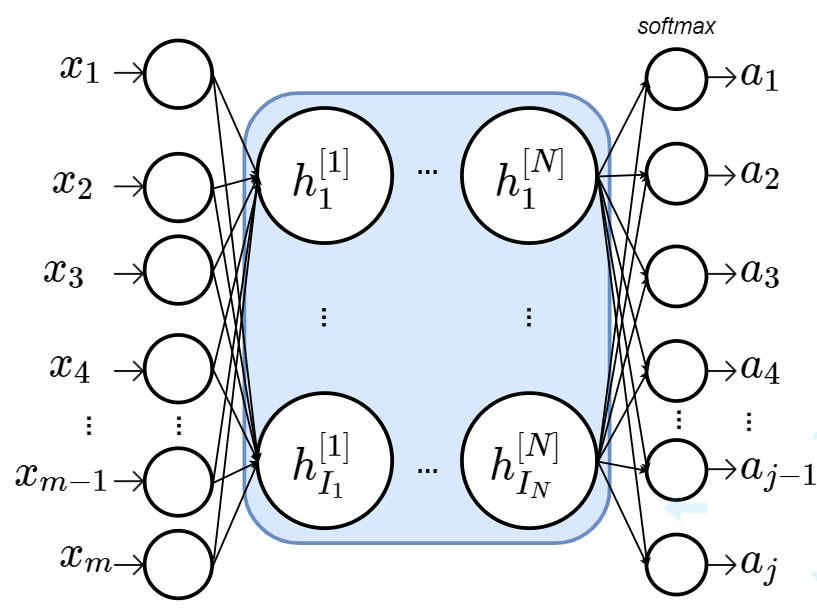
\includegraphics[width=3in]{SimpleNN.png}
    \caption[A simple neural network.]{\label{fig:atomsize} A neural network with $m$ inputs, $j$ outputs,  $N$  hidden layers, and $I$ neurons per layer.}
  \end{figure}
\addtocontents{lof}{\vspace{\normalbaselineskip}}


\pagebreak



%-----------------------------------------------------------------------------------
\section*{CHAPTER II}
%-----------------------------------------------------------------------------------


\vspace{0.25in}
\section{RELATED WORK}
\addtocontents{toc}{\vspace{\normalbaselineskip}}
Deep neural networks have outperformed traditional machine learning approaches for many tasks, and are the tool of choice in many
fields. Specifically, Deep learning has been successfully used for facial recognition \cite{krizhevsky2012imagenet, sun2014deep, ding2015robust}, image classification, 
\cite{simard2003best, ma2015hyperspectral, zhong2011bilinear}, and speech recognition \cite{hinton2012deep, graves2013speech, noda2015audio}, where it is expected to achieve better
performance than humans in the near future. However, directly applying these techniques in fields that deal with private data is
challenging. The reason is that they need to centrally collect data at a third-party which organizations may not trust
\cite{chicurel2000databasing}. This is particularly challenging in medical and financial applications where the privacy of the users is
governed by federal legislation and is protected by law. 

\pagebreak
%-----------------------------------------------------------------------------------
\section*{CHAPTER III}
%-----------------------------------------------------------------------------------
\vspace{0.25in}
\section{DEEP NEURAL NETWORK}
\addtocontents{toc}{\vspace{\normalbaselineskip}}
Deep neural networks are a type of machine learning that has recently shown high accuracy in data classification tasks. Traditional
machine learning requires manual feature selection, which can be time consuming and inaccurate. In contrast, deep learning
learns the most relevant features in the data on its own. In other words, the deep neural networks can be trained with raw data without
the burden of preprocessing it. Since deep neural networks have more hidden layers compared to traditional neural networks, their
accuracy is proportional to the amount of data used for training, i.e., the larger the training data set the more accurate that the
deep neural networks become. These advantages make deep neural networks a very effective technique to perform data classification
tasks. In this section, we describe the architecture of deep neural networks and their training methods. 



%-----------------------------------------------------------------------------------
\subsection{Architecture}\label{sec:MLP}
%-----------------------------------------------------------------------------------

In this work, we consider multilayer perception (MLP), which is one of the most common deep neural network architectures. An
MLP is formed by multiple layers where each layer consists of many nodes. Each node takes 
as input a weighted average of the previous layer's node outputs, and the output of an special node called the bias.  
The nodes use a non-linear activation function to the compute their output. Together, the weights used in the weighted average and
the biases from the special neurons are called the parameters of the deep neural network.


Figure \ref{fig:SimpleNN} shows the structure of a typical classification MLP with $m$ input nodes and $j$ outputs nodes. The neural network
has $N$ hidden layers and each layer has $I$ neurons. Intuitively, this MLP takes a data sample represented as a vector of length
$m$ on its input layer, and outputs the probability that it belongs to the $j$th category on the $j$th output neuron.


\begin{equation}
a^i_k=f(W_k a_{k-1})
\end{equation}
\noindent

\bigskip

%---------------------------------------------------------------------
\subsection{Training}
%---------------------------------------------------------------------
Before a neural network can be used to perform inference, e.g., classify images, it needs to be trained to learn the highly non-linear
relationships between the inputs and the correct outputs. Training finds the 
parameters of the deep neural network, i.e., its the weights and biases, that result in the inferences with the highest accuracy.


%---------------------------------------------------------------------
\subsubsection{Gradient Descent Algorithm}
%---------------------------------------------------------------------
The GD algorithm finds the parameter updates in two steps: error forward propagation and back propagation. 

%---------------------------------------------------------------------------------
\subsubsection{Stochastic Gradient Descent}
%---------------------------------------------------------------------------------

Although the GD algorithm is effective at finding the parameters of DNNs, all  training samples in the dataset need to be processed
before a single update is made to the parameters. That is, the algorithm processes the complete training data at each iteration. 
This is computationally intensive and time consuming. 

\pagebreak
%-----------------------------------------------------------------------------------
\section*{CHAPTER IV}
%-----------------------------------------------------------------------------------
\vspace{0.25in}
\section{PROBLEM FORMULATION}
\addtocontents{toc}{\vspace{\normalbaselineskip}}

In this section, we describe our considered collaborative deep learning model, and the threat model. 

%---------------------------------------------------------------------------------
\subsection{System Model} \label{sec:systemModel}
%---------------------------------------------------------------------------------
\begin{figure}[H]
  \centering
    \includegraphics[width=3in]{ClassificationNN.png}
    \caption[A simple neural network.]{\label{fig:ClassNN} Neural network depicting an image with $m \times m$ pixels fed as input, $j$ outputs  $N$  hidden layers and with $I$ neurons in layer.}
  \end{figure}
\addtocontents{lof}{\vspace{\normalbaselineskip}}


%-------------------------------------------------------------------------
\subsection{Privacy-preserving Distributed Learning under the Semi-honest Threat Model}
%-------------------------------------------------------------------------
To allow user $u_0$ to train its deep learning network while preserving the privacy of all users, we could use the distributed
learning approach proposed by Shokri et al. \cite{shokri2015privacy}. This approach allows user $u_0$, as well as the rest of the users, 
to use the private data from each other to train a deep learning model. By only sharing certain parameters of their local models
with a parameter server, it allows them to update their local models without having to transmit any of their samples to each other
or to the their private sets. We assume that the architecture and training parameters of  deep neural network that user $u_0$ aims to
train are known  to all other users and the PS.


%---------------------------------------------------------------------------------
\subsection{A Malicious Threat Model for Distributed Deep Learning}\label{sec:threatModel}
%---------------------------------------------------------------------------------

We consider a malicious threat model for both the parameter server and the users. Specifically, malicious users will
attempt to learn private information about other users' dataset based on the parameters that they uploads.  In
addition, one or multiple  users will upload malicious parameters that can trick a victim user into reveal its private information. 
Such an attack has been described by Hitaj et al. \cite{hitaj2017deep}. In particular, the attack operates as follows. 
Suppose user $u_A\in\mathcal{U}$ is malicious and targets another user $u_V\in\mathcal{U}$. Further assume that all users, including
the malicious one, agree on the hyper parameters of a neural network architecture such as the number, size and type of layers,  and the
classification labels as described in Section \ref{sec:systemModel}.


\pagebreak
%-----------------------------------------------------------------------------------
\section*{CHAPTER V}
%-----------------------------------------------------------------------------------
\vspace{0.25in}
\section{A PRIVACY-PRESERVING COLLABORATIVE LEARNING ALGORITHM}
\addtocontents{toc}{\vspace{\normalbaselineskip}}



\begin{figure}[H]
  \centering
    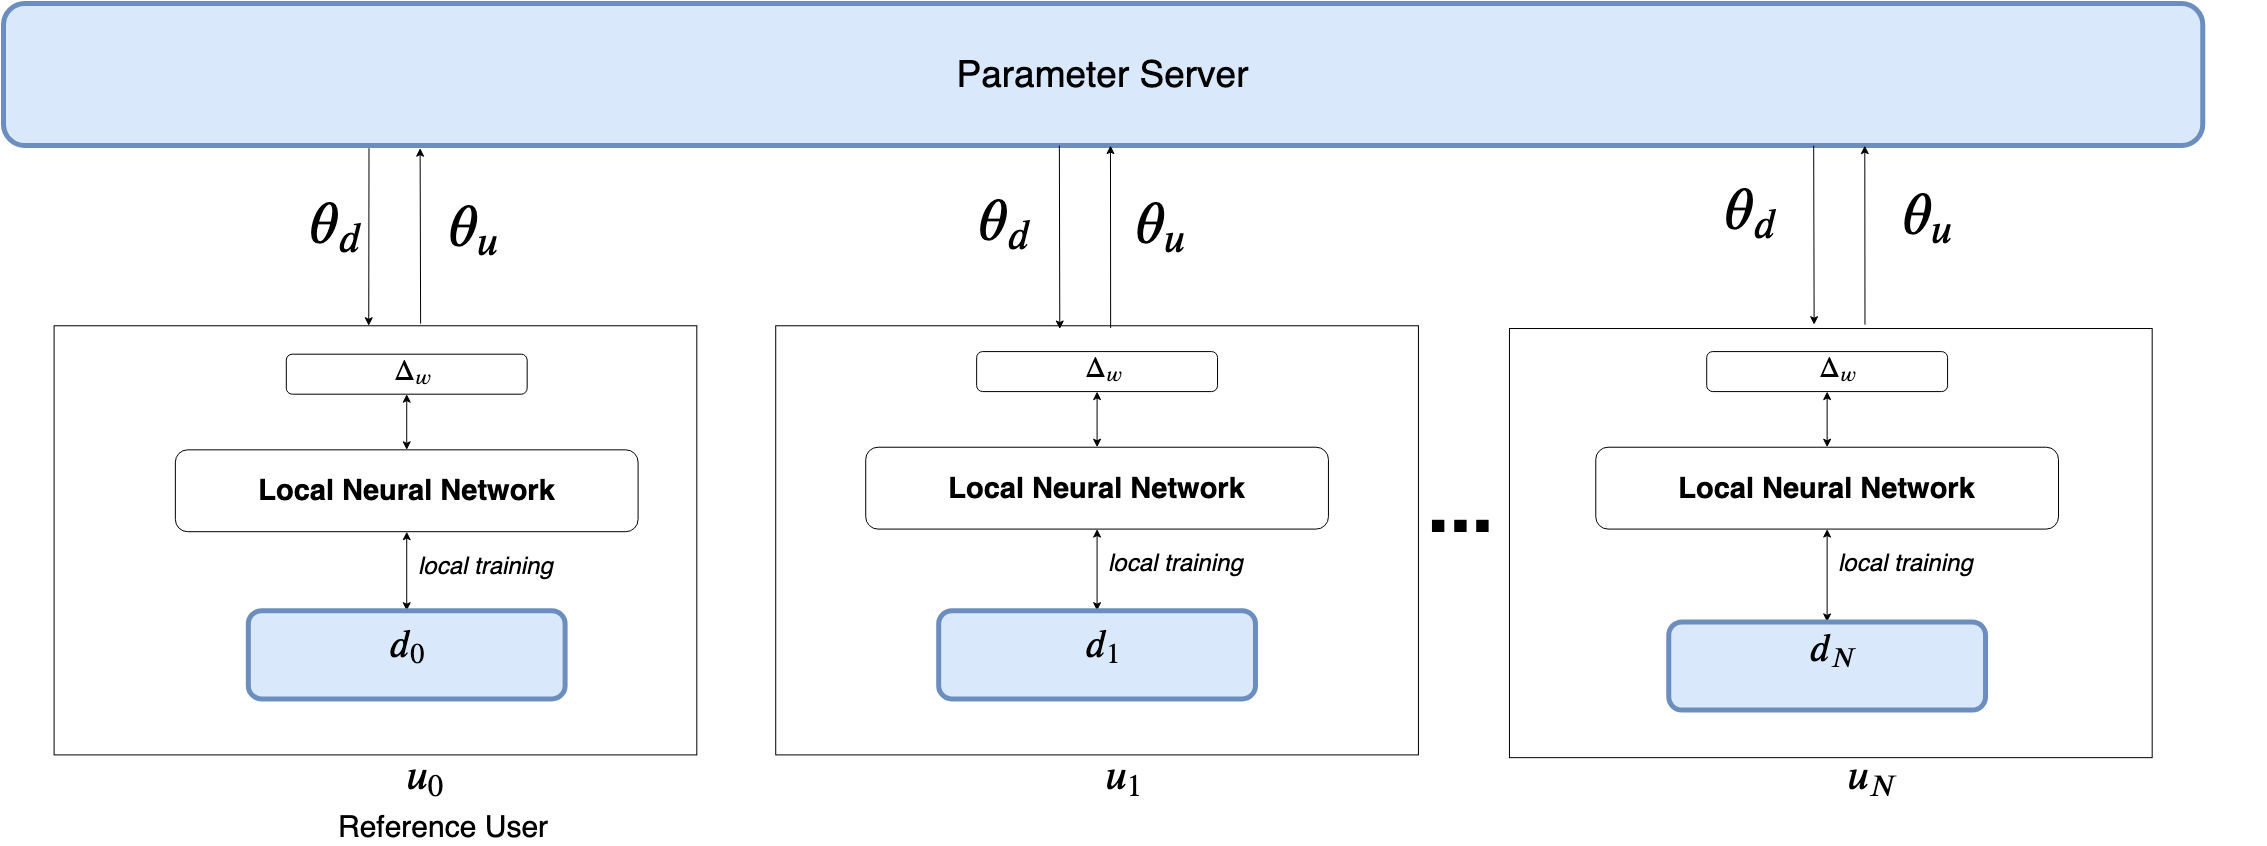
\includegraphics[width=3in]{HighLevelArch.png}
    \caption[A privacy preserving architecture.]{\label{fig:HighLevel} An architecture for privacy-preserving distributed learning.}
  \end{figure}
\addtocontents{lof}{\vspace{\normalbaselineskip}}



In this section we describe our proposed privacy-preserving distributed learning algorithm. Our approach prevents attacks such as the ones described in Section \ref{sec:threatModel} by limiting the amount of times users can upload parameters to the servers. 

%Our proposed algorithm prevents attacks such as the one proposed in \cite{hitaj2017deep}. 
In specific, we protect the participants from GAN based attacks by preventing an innocent user from parameter sharing in a predictable and repeated way which reduces the adversarial influence as described in \cite{hitaj2017deep}.  We randomly choose the set of participants that can interact with the server at one time period called the round, $r$. This randomized choosing of participants reduces the chances of selecting the malicious participant in every round. It impacts the adversary because it can no longer upload its malicious parameters to the server forcing innocent participants to reveal more of their private dataset.

Specifically, our approach is as follows. We suppose all participants in the architecture agree on the hyper parameters such as classification labels, type and architecture of neural networks.
All participants data sets from all users are considered private information that needs to be protected from other users and the parameter server. We also consider a user $u_0$ who aims to train a local deep neural network using its local training data set as well as the training data sets from other users as described in Section \ref{sec:systemModel}. 
We then select a random subsection of the participants that can take turns to interact with the server such that only one participant interacts with the server at one time. The selected participants downloads some fraction of parameters, $\theta_d$, from the server. A selected participant, $u_i$  overwrites their corresponding local parameters with downloaded parameters. It then trains their network privately on local datasets, $d_i$. $u_i$ then individually upload the their largest parameter gradients, $\theta_u$,  to the parameter server, which aggregates them.
The selected participant uploads trains and downloads the parameters over a specific number of epoch, before the next selected participant can interact with the server.
At the end, when all selected participants have completed their interaction, reference user $u_0$ can downloads the parameters from the server train further train its local network. In this way, $u_0$ never uploads its parameters to the server and does not reveal any private data. 


Formally,the algorithm is as follows:
\begin {enumerate}
\item Out of all available participants, a random subsection of participants is selected to interact with the parameter server in this
period. We call this period a round which is denoted by $r$. In each round, $r_i$, the selected users are able to interact with the parameter exclusively such that no two
participants can interact with the parameter server at the same time.
\item During its interaction with parameter server, a selected user $u_i$ will perform the following steps:
\begin {enumerate}
  \item Train independently on its local dataset for one epoch, to calculate parameter gradient, $\Delta w_i$ 
  \item  At the end of the epoch, $u_i$ will select the $\theta_u$ fraction of highest gradients in its local $\Delta w$. It will then upload that fraction of values in $\Delta w_i$ to the parameter server.
  \end {enumerate}
\item For each subsequent epoch, the participant will first download $\theta_d$ percentage of parameters from the server. The
user will then repeat the steps a and b. We repeat these steps for every participant selected in $r_i$.
\item At the end of $r_i$, the reference user downloads $\theta_d$ percentage of parameters from the parameter server.
\item The reference user, $u_0$, then trains its model locally on its dataset. 
\end {enumerate}



\pagebreak
%-----------------------------------------------------------------------------------
\section*{CHAPTER VI}
%-----------------------------------------------------------------------------------
\vspace{0.25in}
\section{A PRIVACY-PRESERVING COLLABORATIVE LEARNING ALGORITHM}
\addtocontents{toc}{\vspace{\normalbaselineskip}}
%-------------------------------------------------------------------------------
\section{EXPERIMENTAL SETUP}
%-------------------------------------------------------------------------------

To evaluate the performance of our proposed privacy-preserving approach, we implement it on a commercial cloud service provider, and measure the
learning performance of the user $u_0$, and compare it to the learning performance of a centralized deep neural network
architecture, and to the distributed learning architecture proposed by Shokri et al. \cite{shokri2015privacy}.

\begin{figure}[H]
  \centering
    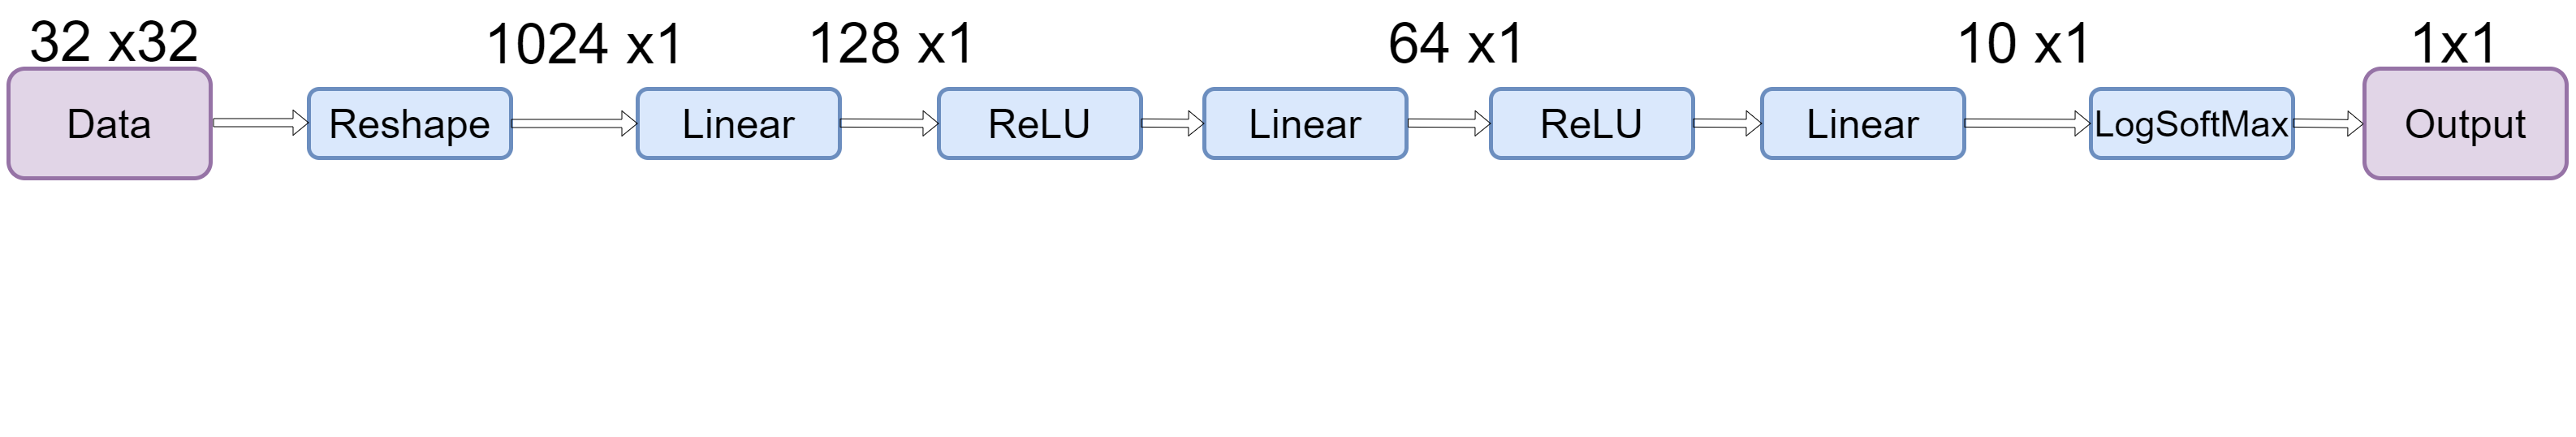
\includegraphics[width=3in]{MLPArchitecture.png}
    \caption[Tensor sizes in a MLP architecture.]{\label{fig:MLPArch} MLP architecture displaying the tensor size at various stages in the neural network..}
  \end{figure}
\addtocontents{lof}{\vspace{\normalbaselineskip}}


%-------------------------------------------------------------------------------
\subsection{Datasets}
%-------------------------------------------------------------------------------
We conducted our experiments using the MNIST dataset \cite{deng2012mnist}. The MNIST dataset is a standard dataset used in image
recognition. It contains images of hand-written gray scale digits ranging from 0 to 9. The dimension of each image is 32 X 32 pixels.
The MINST dataset contains 60,000 images in its training dataset and 10,000 images in its test dataset.
For this experiment, we center the images through a normalization operation.  

%--------------------------------------------------------------------------------------------
\subsection{Hyper-parameter Setup}

%--------------------------------------------------------------------------------------------

Hyper-parameters are parameters that control the collaborative learning process, e.g., learning rate $\alpha$, fraction of upload and download gradients $\theta_u$ and $\theta_d$ respectively. Unlike
the deep neural network parameters that are obtained through training, hyper parameters are usually set beforehand and remain
constant through out the training and inference phases. They are crucial since they directly influence the behaviour of training
algorithm and have a large impact on the performance and accuracy of the model. In our experiments, we set the learning rate $\alpha$ for all
users to $0.1$. 
The mini-batch size $M$ for stochastic gradient descent training is set to 10 samples.


\pagebreak
%-----------------------------------------------------------------------------------
\section*{CHAPTER VI}
%-----------------------------------------------------------------------------------
\vspace{0.25in}
\section{EXPERIMENT RESULTS}
\addtocontents{toc}{\vspace{\normalbaselineskip}}


\begin{figure}[H]
  \centering
    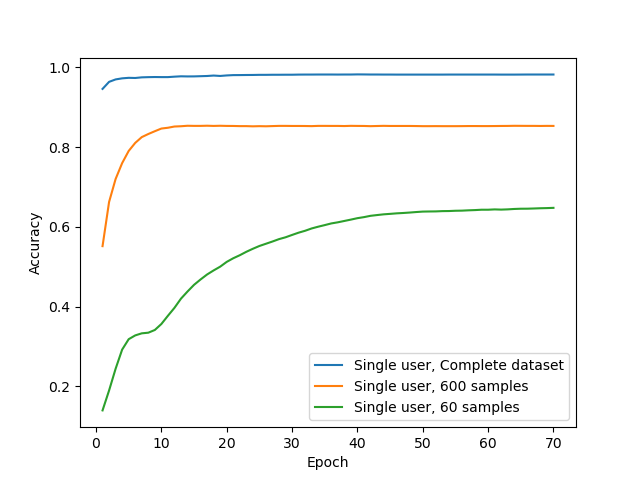
\includegraphics[width=3in]{SingleUserBaselines.png}
    \caption[Single User with varying sample size.]{\label{fig:SingleUser} Single User with varying sample size}
  \end{figure}
\addtocontents{lof}{\vspace{\normalbaselineskip}}

To fairly assess the performance improvements offered by our proposed privacy-preserving algorithm, we first measure the accuracy of
the centralized approach, i.e., a single entity who collects the data from all users but does not provide privacy. 
Figure \ref{fig:SingleUser} shows the accuracy of the centralized approach for a varying number of epochs. As expected, we see that
that the accuracy obtained by the centralized approach increases with the number of epochs. 
Moreover, to assess the impact of users who only have access to their local data set and do not participate in distributed
learning, we measure the accuracy for different sizes of the training data set. We see that the accuracy decreases with the number
of samples in the data set. This confirms that a small local data set can only provide a low accuracy to the reference user $u_0$.

\begin{figure}[H]
  \centering
    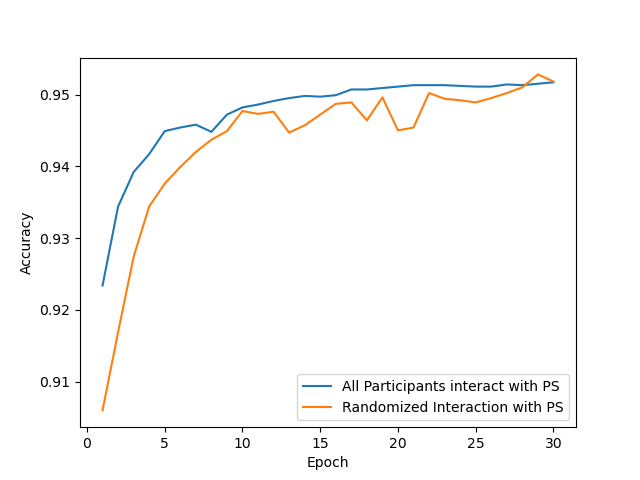
\includegraphics[width=3in]{RandomVsAll.png}
    \caption[Comparison between randomized interaction and complete interaction with server.]{\label{fig:RandVsAll} Comparison between randomized interaction and complete interaction with server}
  \end{figure}
\addtocontents{lof}{\vspace{\normalbaselineskip}}



Next, we compare the accuracy of the reference user under our proposed privacy-preserving algorithm and that of the algorithm proposed
by Shokri et al. \cite{shokri2015privacy}. Figure \ref{fig:RandVsAll} shows the accuracy of the reference user $u_0$'s deep learning
neural network trained under our proposed deep learning algorithm, and under \cite{shokri2015privacy}. We set the number of
users to 20 for both approaches. In our approach, each of the non-reference users $u_i$ is randomly
selected to upload and download parameters from the parameter server with a probability of 0.5. 


\begin{figure}[H]
  \centering
    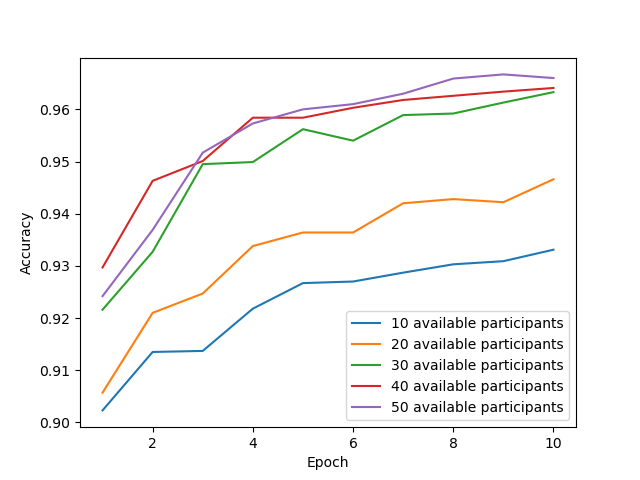
\includegraphics[width=3in]{VaryingPoolofParticipants.png}
    \caption[Distributed SGD for varying participant.]{\label{fig:VaryingPoolofParticipants} Accuracy of Distributed SGD for varying participants available for interaction with the PS.}
  \end{figure}
\addtocontents{lof}{\vspace{\normalbaselineskip}}



Figure \ref{fig:VaryingPoolofParticipants} shows the accuracy of the reference users $u_0$'s deep neural network under a varying number of epochs for different numbers of total users in the system. We observe that 
the reference user $u_0$ achieves a higher accuracy as the total number of participants in the system increases. For example, the
highest accuracy is achieved with 50 participants, while the lowest one is achieved with 10 participants. Intuitively, this is bebacuse the greater number of participants bring a larger size and variety of dataset. This means the parameters uploaded to the server increases with the number of users. improving the accuracy of the model.



\begin{figure}[H]
  \centering
    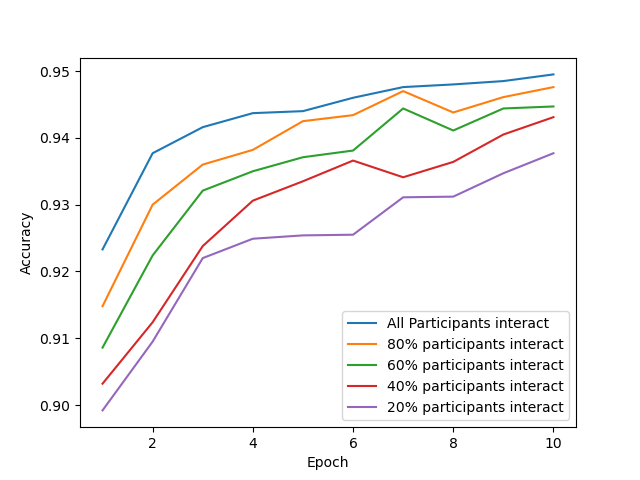
\includegraphics[width=3in]{VaryingProbabilityInteraction.png}
    \caption[SGD for varying probability of interaction.]{\label{fig:VaryingProbabilityInteraction} Accuracy of Distributed SGD for varying probability of interaction with the PS.}
  \end{figure}
\addtocontents{lof}{\vspace{\normalbaselineskip}}


Figure \ref{fig:VaryingProbabilityInteraction} shows the accuracy of reference user $u_0$ for a varying number of epochs under
different probabilities for the users to interact with the parameter server. 
We see that a greater probability of interaction with the server results in a higher model accuracy for the reference user $u_0$.
The highest accuracy is obtained when all participants interact with the parameter server. However, this is equivalent to the
approach proposed by \cite{shokri2015privacy} and thus it is vulnerable to the attacks described in \cite{hitaj2017deep}. 


\begin{figure}[H]
  \centering
    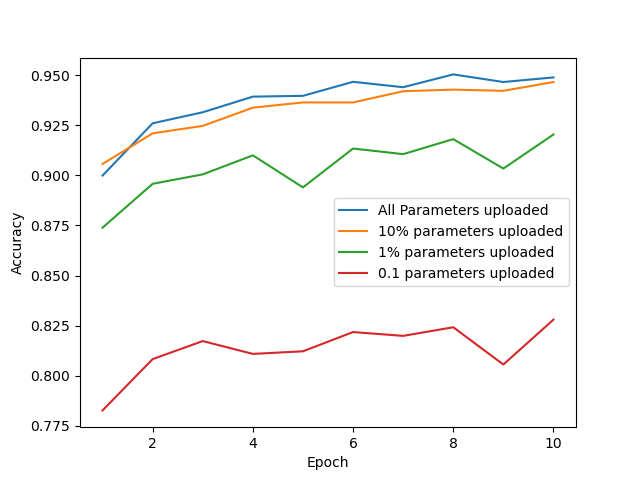
\includegraphics[width=3in]{VaryingThetaU.png}
    \caption[Different upload gradient selection rate]{\label{fig:VaryingThetaU}Accuracy of Distributed SGD for different upload gradient selection rate, unevenly.}
  \end{figure}
\addtocontents{lof}{\vspace{\normalbaselineskip}}



Figure \ref{fig:VaryingThetaU} we plot the accuracy of the reference user $u_0$ for different upload gradient selection rate over. 
The plot shows that the percentage of uploaded parameters, $\theta_u$, is directly proportional to the resulting accuracy of
the model at $u_0$. However, the accuracy difference between the sharing all parameters and only $ 10\% $ percent of parameters is
insignificant.





\pagebreak
%-----------------------------------------------------------------------------------
\section*{CHAPTER III}
%-----------------------------------------------------------------------------------
\vspace{0.25in}
\section{CONCLUSION}
In this work we propose, implement and analyse a secure privacy preserving approach to distributed deep learning systems.  Our algorithm provides security against attacks that extract information from participants in a collaborative setting. 

Our work can be extremely beneficial in providing a secure application of distributed and decentralized collaborative learning. This will make it more accessible to users concerned about their privacy but want to benefit from larger datasets.

Our methodology provides countermeasure to the category of attacks that use malicious parameters to influence victims to reveal more information as described  by Hitaj  et al. \cite{hitaj2017deep} . We do this by limiting the consistent exposure of each participant to the server and to other users.
Our solution does not rely on computationally expensive cryptographic process and has a adaptable architecture that can be used with any underlying neural network structure.
For the scope of this work we assume that the multiple users and the parameters are non-colluding and only share information outlined by our protocol. 

\newpage

\begin{center}
\vspace*{\fill}
\addcontentsline{toc}{section}{BIBLIOGRAPHY}
\section*{\normalfont BIBLIOGRAPHY}
\vspace*{\fill}
\end{center}
\newpage
\let\oldaddcontentsline\addcontentsline% Store \addcontentsline
\renewcommand{\addcontentsline}[3]{}% Remove functionality of \addcontentsline
\renewcommand\bibname{\normalfont BIBLIOGRAPHY}
\bibliography{sample}
\let\addcontentsline\oldaddcontentsline% Restore \addcontentsline

%%%%%%%%%%%%%%%%%%%%%%%%%%%%Appendix%%%%%%%%%%%%%%%%%%%%%%%%%%%%%%%%
\newpage
\appendix
\addcontentsline{toc}{section}{APPENDIXES}
\addtocontents{toc}{\vspace{\normalbaselineskip}}
\renewcommand\thesubsection{\Alph{subsection}}
\newpage

\begin{center}
\vspace*{\fill}
\section*{\normalfont APPENDIXES}
\vspace*{\fill}
\end{center}

%%%%%%%%%%%%%%%%% Appendix A %%%%%%%%%%%%%%%%%%%%%%%
\newpage
\section*{\normalfont APPENDIX A} \label{App:A}
\section*{Possible Alter Egos} 
\addcontentsline{toc}{subsection}{A. Possible Alter Egos}
\addtocontents{toc}{\vspace{\normalbaselineskip}}
Possible alter egos to facilitate crime fighting: Ant-Man, Giant Man, Quantum-Man, The Wasp, The Whisper. 

%%%%%%%%%%%%%%%%% Appendix B %%%%%%%%%%%%%%%%%%%%%%%
\newpage
\section*{\normalfont APPENDIX B} \label{App:B}
\section*{My Awesome Suit} 
\addcontentsline{toc}{subsection}{B. My Awesome Suit}
\addtocontents{toc}{\vspace{\normalbaselineskip}}

Here's a look at my awesome suit. 

}

\end{flushleft}
\end{document}
